%%%% This CV has been greatly influence by
%%%% the extended fancy cv from Carmine Benedetto.
%%%% I thank him for the excellent work. Unfortunately 
%%%% it wouldn't compile on my machine. So I worked it out myself.

\documentclass{article} 
\usepackage[ngerman]{babel}% deutsche Trennregeln
\usepackage{microtype}% verbesserter Randausgleich
\usepackage[utf8]{inputenc}
\usepackage{graphicx}
\usepackage{color}
\usepackage[svgnames]{xcolor}
\usepackage[obeyspaces]{url} 


\usepackage{calc}

% define margin
\newlength\cvMargin
\setlength\cvMargin{0.25cm}

\usepackage[margin=\cvMargin,noheadfoot,a4paper]{geometry}

% other lengths
\newlength\cvSideWidth
\setlength\cvSideWidth{0.27\paperwidth-\cvMargin}

\newlength\cvMainWidth
\setlength\cvMainWidth{\paperwidth-4\cvMargin-\cvSideWidth}

\newlength\cvPictureWidth
\setlength\cvPictureWidth{4cm}

\newlength\cvLanguageBarWidth
\setlength\cvLanguageBarWidth{5em}

\newlength\cvLanguageBarHeight
\setlength\cvLanguageBarHeight{0.75em}


%\usepackage[left=0cm,top=0cm,right=0cm,bottom=0cm,nohead,nofoot]{geometry}
%\usepackage[a4paper,left=0cm,top=0cm,right=0cm,bottom=0cm,nohead,nofoot]{geometry}

\usepackage{fontawesome}


\usepackage{blindtext}
%\usepackage{setspace}
%%\onehalfspacing
%\setstretch{1.1}

\usepackage{pdfcomment}
%% Fix incorrect display of tooltips (http://tex.stackexchange.com/a/74340/3323)
\makeatletter
\renewcommand{\pc@annot@tooltip}%
{%
  /TU (\pc@pdfenc@contents)\space%
  /T (tooltip \thezref@unique)\space%
  /C [0 0 0]\space%
  /FT/Btn\space%
  /Ff 65536\space%
  /H/N\space%
}%

\setlength{\parindent}{0pt}
\setlength{\fboxsep}{10pt}
\setlength{\fboxrule}{20pt}

\makeatletter
\def\cv@hrulefill{{\color{pblue}\leavevmode\leaders\hrule height 1pt\hfill\kern\z@}}

% line before and after text
\NewDocumentCommand{\ruleline}{m}{\par\noindent\raisebox{\baselineskip/4}{\makebox[\linewidth]{\cv@hrulefill\hspace{1ex}\raisebox{-\baselineskip/4}{#1}\hspace{1ex}\cv@hrulefill}}}
\makeatother


\newcommand{\spacingWork}{0.25cm}

\definecolor{white}{RGB}{255,255,255}
\definecolor{anti-flashwhite}{rgb}{0.95, 0.95, 0.96}

\definecolor{darkgray}{HTML}{333333}
\definecolor{gray}{HTML}{4D4D4D}
\definecolor{lightgray}{HTML}{999999}

\definecolor{green}{HTML}{C2E15F}
\definecolor{orange}{HTML}{FDA333}
\definecolor{purple}{HTML}{D3A4F9}
\definecolor{red}{HTML}{FB4485}
\definecolor{blue}{HTML}{6CE0F1}
\definecolor{pblue}{HTML}{0395DE}
% define four main colours
\definecolor{cvGreen}{HTML}{357F2D}
\definecolor{cvGreenLight}{HTML}{B8E4B3}
\definecolor{cvDark}{HTML}{2F3142}

\usepackage{tikz}
\usetikzlibrary{calc,positioning,backgrounds,matrix}

% set TikZ styles
\tikzset{
  contactIcon/.style={%
    minimum height=\baselineskip,
  },
  contactText/.style={%
    minimum height=\baselineskip,
    text depth=0pt,
  },
  languageText/.style={},
  progressArea/.style={%
    draw,
    rectangle,
    minimum width=\cvLanguageBarWidth,
    minimum height=\cvLanguageBarHeight,
    pblue},
  progressBar/.style={%
    minimum height=\cvLanguageBarHeight,
    rectangle,
    draw,
    fill,
    pblue,
    anchor=west},
  }

\newcommand*{\ClipSep}{0.1cm}%

\renewcommand{\thempfootnote}{\arabic{mpfootnote}}

\usepackage{hyperref}
\hypersetup{
    pdftitle={},
    pdfauthor={},
    pdfsubject={},
    pdfkeywords={},
    colorlinks=false,       % no lik border color
   allbordercolors=white    % white border color for all
}

\pagestyle{empty}

% update default paragraph indent, and header space
\setlength{\topskip}{0pt}      % between header and text (0 needed for vertical centring)
\usepackage{parskip}           % remove paragraph indents


%%%%%%%%%%%%%%%%%%%%%%%%%%%%%%%%%%%%%%%%%%%%%%%%%%%%%%%%%%%%%%%%%%%%%%%%%%%%%%%%%%%%%%%%%%%%%%

\begin{document}
\begin{tikzpicture}[remember picture,overlay]
  \fill[anti-flashwhite] (current page.north west) 
    rectangle ++(\cvSideWidth+2\cvMargin,-\paperheight);
\end{tikzpicture}
\begin{minipage}{0.25\textwidth}
\vspace*{\fill}
  \begin{center}
  \begin{tikzpicture}
    \node[
      circle,
      minimum size=\cvPictureWidth,
      path picture={
        \node at (path picture bounding box.center){
        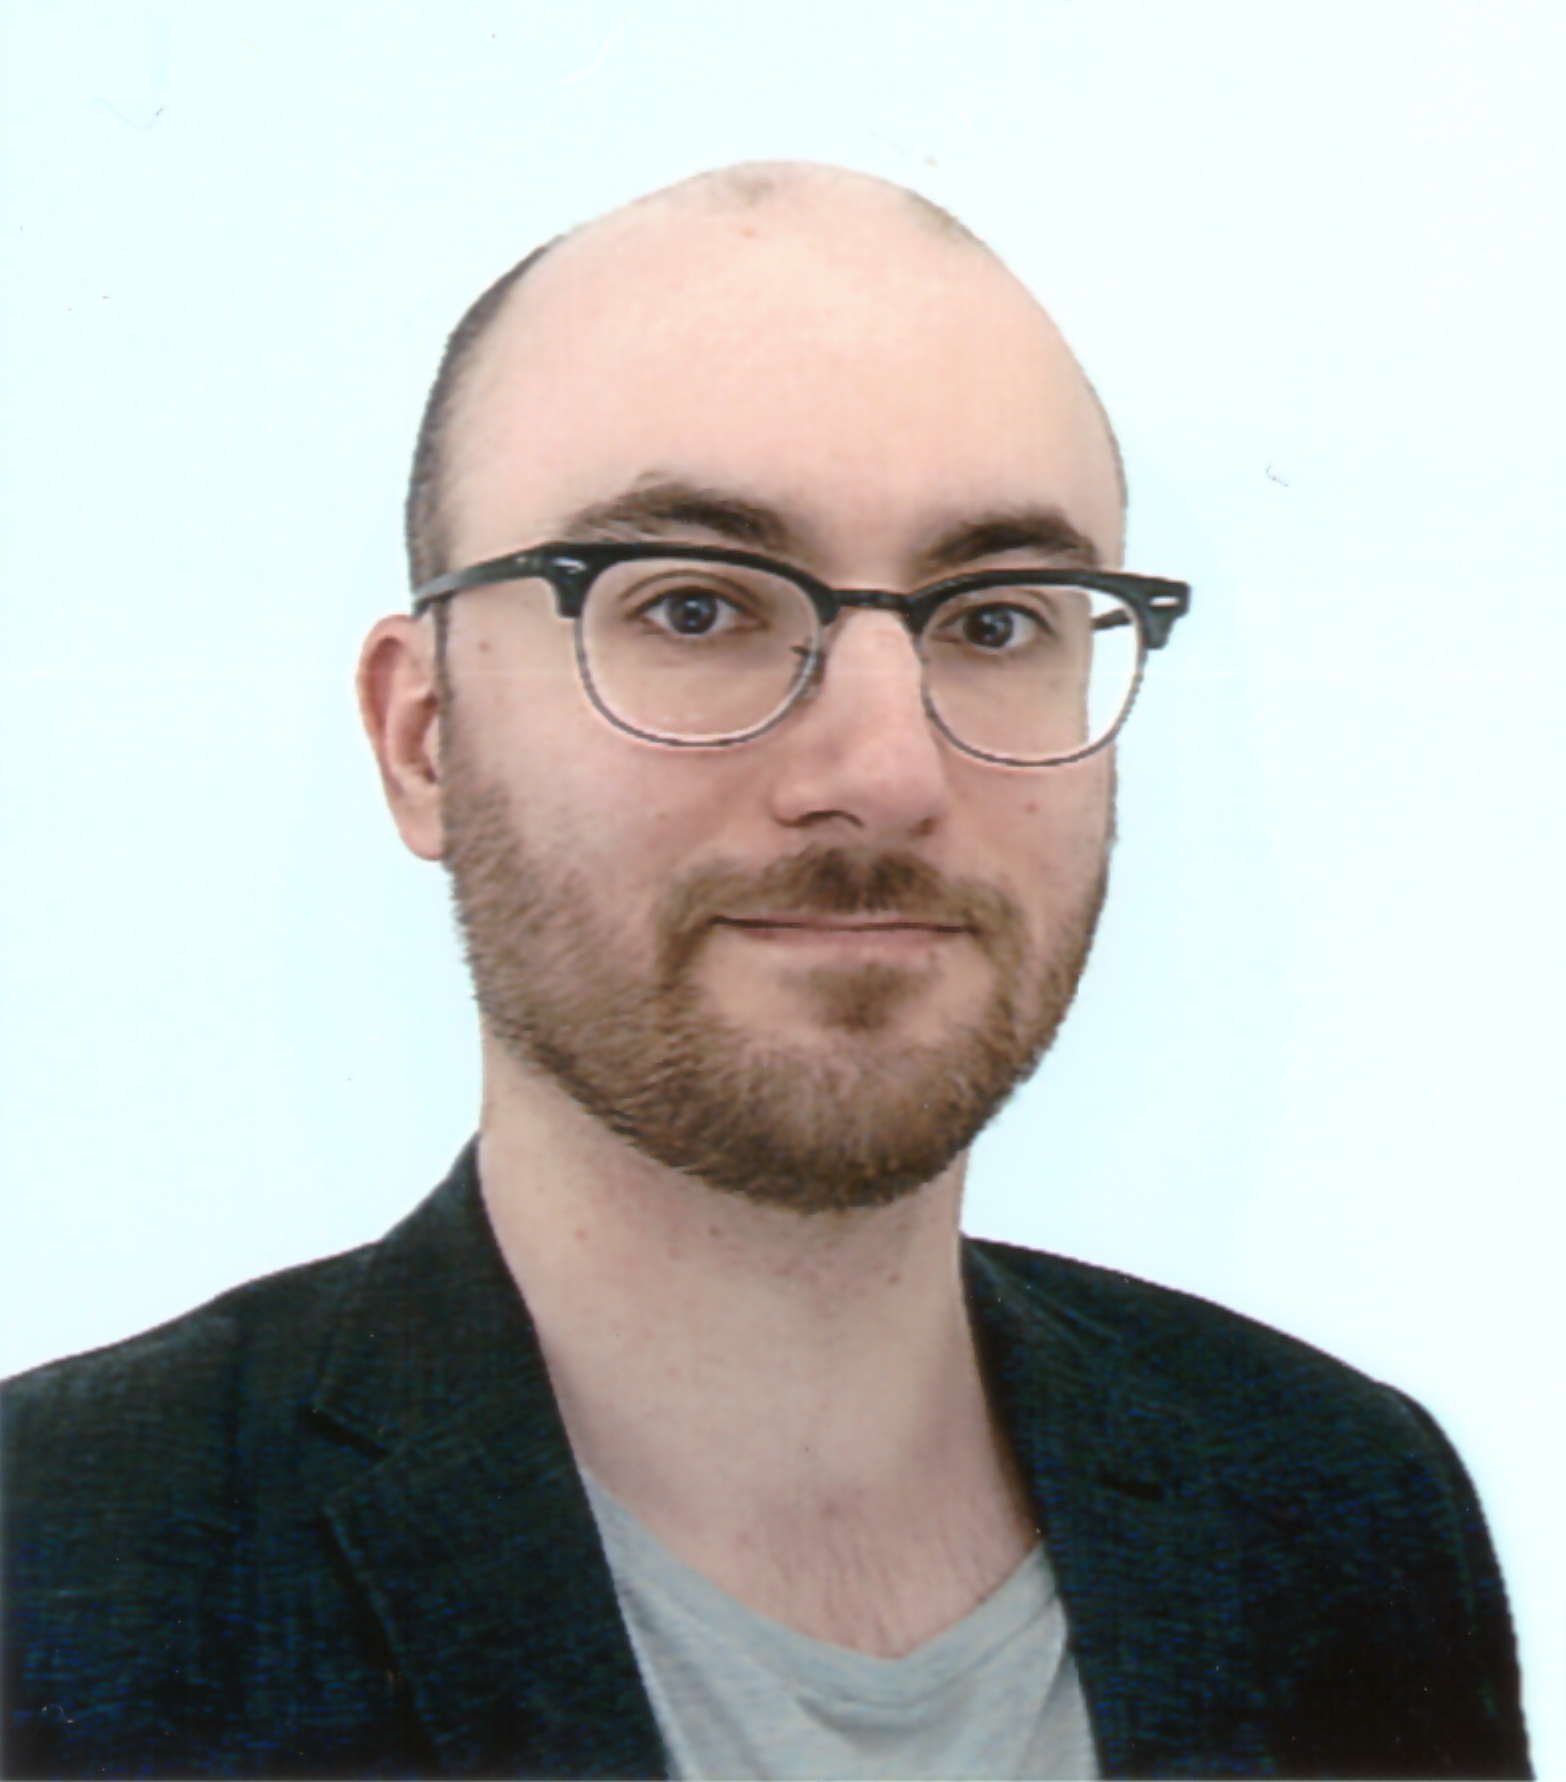
\includegraphics[width=\cvPictureWidth]{../../img/cvImg.png}
        };
      }]
      {};
  \end{tikzpicture}

	{\color{pblue}\faMapMarker}~ Potsdam, Deutschland\\

	\vspace{0.15cm}
	{\color{pblue}\faPhone}	+49 174/6507598

	\vspace{0.15cm}
	{\color{pblue}\faEnvelope}~\href{mailto:silvio{\_}schwarz@web.de}{silvio{\_}schwarz@web.de}%\href{mailto:admin@silvioschwarz.com}{admin@silvioschwarz.com}\\

	\vspace{0.25cm}

	{\Large\color{pblue}\faGithub}~\href{https://github.com/silvioschwarz}{github.com/silvioschwarz}
		\vspace{2mm}

%	\section*{\fontsize{18pt}{24pt}\selectfont \color{pblue} Programmierung}
%	\vspace{0.5mm}
%	\textbf{\LARGE \faLinux}
\includegraphics[scale=0.50]{../../img/5stars.png}\\
%	\textbf{\LARGE \faWindows}
\includegraphics[scale=0.50]{../../img/3stars.png}\\
%	\vspace{5mm}
%
%	\begin{tikzpicture}[node distance = 7mm, terminal/.style={
%					rectangle, minimum height = 2mm, rounded corners = 1mm, thick,
%					draw = darkgray, fill = white, align = left}]
%		\node (A) [terminal] {Python};
%		\node (AA) [terminal, right=2mm of A.east,anchor=west] {R};
%		\node (AAA) [terminal, right=2mm of AA.east,anchor=west] {Matlab};
%		\node (C) [terminal, below=of A.west,anchor=west] {Mathematica};
%		\node (CC) [terminal, right=2mm of C.east,anchor=west] {Latex};
%		\node (D) [terminal, below=of C.west,anchor=west] {HTML/CSS/JS};
%		\node (DD) [terminal, right=2mm of D.east,anchor=west] {ArcGIS};
%		\node (E) [terminal, below=of D.west,anchor=west] {BASH};
%		\node (F) [terminal, right=2mm of E.east,anchor=west] {QGIS};
%		\node (FF) [terminal, right=2mm of F.east,anchor=west] {Git/GitHub};
%		\node (G) [terminal, below=of E.west,anchor=west] {GMT};
%		\node (GG) [terminal, right=2mm of G.east,anchor=west] {Tensorflow};
%		\node (GGG) [terminal, right=2mm of GG.east,anchor=west] {PyTorch};
%	\end{tikzpicture}
%
%	\vspace{3mm}
%	%\includegraphics[scale=0.3]{../../../img/Programmierung.pdf}
%
%	\hrule
%	\vspace{-2mm}
%	\section*{\fontsize{18pt}{24pt}\selectfont \color{pblue} Sprachen}
%	\vspace{-2mm}
%	\center
%	\begin{itemize}
%		\centering
%		\item[\textbf{Deutsch}] 
\includegraphics[trim=0cm 0.2cm 0cm 0cm, clip,scale=0.50]{../../img/5stars.png}\vspace{-2mm}
%		\item[\textbf{Englisch}]  
\includegraphics[trim=0cm 0.15cm 0cm 0cm, clip,scale=0.50]{../../img/4stars.png}\vspace{-2mm}
%		\item[\textbf{Italienisch}] 
\includegraphics[trim=0cm 0.2cm 0cm 0cm, clip,scale=0.5]{../../img/3stars.png}\vspace{-2mm}
%		\item[\textbf{Französisch}]  
\includegraphics[trim=0cm 0.2cm 0cm 0cm, clip,scale=0.50]{../../img/2stars.png}
%	\end{itemize}
%	\hrule
%	\vspace{-2mm}
\ruleline{Sprachen}

\vspace{4pt}

\begin{tikzpicture}[every node/.style={text depth=0pt,inner sep=0pt,outer sep=0pt}]
  \matrix [
    column 1/.style={anchor=east,languageText},
    column 2/.style={anchor=west,align=left,progressArea},
    column sep=6pt,
    row sep=6pt,
    ] (contact) {
    \node{Deutsch}; & \node (language 1) {}; \\
    \node{Englisch};  & \node (language 2) {}; \\
    \node{Italienisch}; & \node (language 3) {}; \\
  };
  \draw (language 1.west) node[progressBar,minimum width=5/5*\cvLanguageBarWidth] {};
  \draw (language 2.west) node[progressBar,minimum width=3/5*\cvLanguageBarWidth] {};
  \draw (language 3.west) node[progressBar,minimum width=3/5*\cvLanguageBarWidth] {};
\end{tikzpicture}
%	\section*{\fontsize{18pt}{24pt}\selectfont \color{pblue} Expertise}
%	\vspace{-0.2mm}
%	\begin{tikzpicture}[node distance = 7mm, terminal/.style={
%					rectangle, minimum height = 2mm, rounded corners = 1mm, thick,
%					draw = darkgray, fill = white, align = left}]
%		\node (A) [terminal] {seismische Gefährdungsanalyse};
%		\node (AAA) [terminal,  below=of A.west,anchor=west] {machine learning};
%		\node (AAB) [terminal,  right=2mm of AAA.east,anchor=west] {deep learning};
%		\node (AAAA) [terminal,  below=of AAA.west,anchor=west] {Bayes'sche Methoden };
%		\node (C) [terminal,  below=of AAAA.west,anchor=west] {Zeitreihenanalyse};
%	\end{tikzpicture}
%	\vspace{-2mm}
%	\hrule
%	\vspace{-2mm}
%	\section*{\fontsize{18pt}{24pt}\selectfont \color{pblue} Zertifikate}
\ruleline{Zertifikate}

\vspace{4pt}

	\centering
	\vspace{-2mm}
	\textbf{\color{pblue}\underline{Tensorflow}}\\
	\href{https://www.coursera.org/account/accomplishments/specialization/certificate/WNXPGV8FR3AF}{\color{pblue}Developer},
	\href{https://www.coursera.org/account/accomplishments/specialization/certificate/R4LSQ7AK8M83}{\color{pblue}Data and Deployment},
	\href{https://www.coursera.org/account/accomplishments/specialization/certificate/5DDY3GKK3YTV}{\color{pblue}Advanced Techniques},
	\href{https://www.coursera.org/account/accomplishments/specialization/certificate/KA3YGBWN8RM2}{\color{pblue}Generative Adversarial Networks (GANs)},
	\href{https://www.coursera.org/account/accomplishments/certificate/JKHKJWYFUT43}{\color{pblue}Natural Language Processing (NPL)},
	\href{https://www.coursera.org/account/accomplishments/specialization/certificate/SCJJ3AWTKR4B}{\color{pblue}Machine Learning Engineering for Production (MLOps)}\\
	
	\textbf{\color{pblue}\underline{Google}}\\
	\href{https://www.coursera.org/account/accomplishments/specialization/certificate/U9C59W5MS826}{\color{pblue}Google IT Support}\\
	
	\textbf{\color{pblue}\underline{Stanford University}}\\
	\href{https://www.coursera.org/api/legacyCertificates.v1/spark/statementOfAccomplishment/972304~5332413/pdf}{\color{pblue}Machine Learning}\\
	
	\textbf{\color{pblue}\underline{IBM}}\\
	\href{https://www.coursera.org/account/accomplishments/certificate/JNSWNP2SMB6A}{\color{pblue}IBM Full Stack-Cloudentwickler}

	\centering
%	\section*{\fontsize{18pt}{24pt}\selectfont \color{pblue} Interessen}
\ruleline{Interessen}
\vspace{4pt}
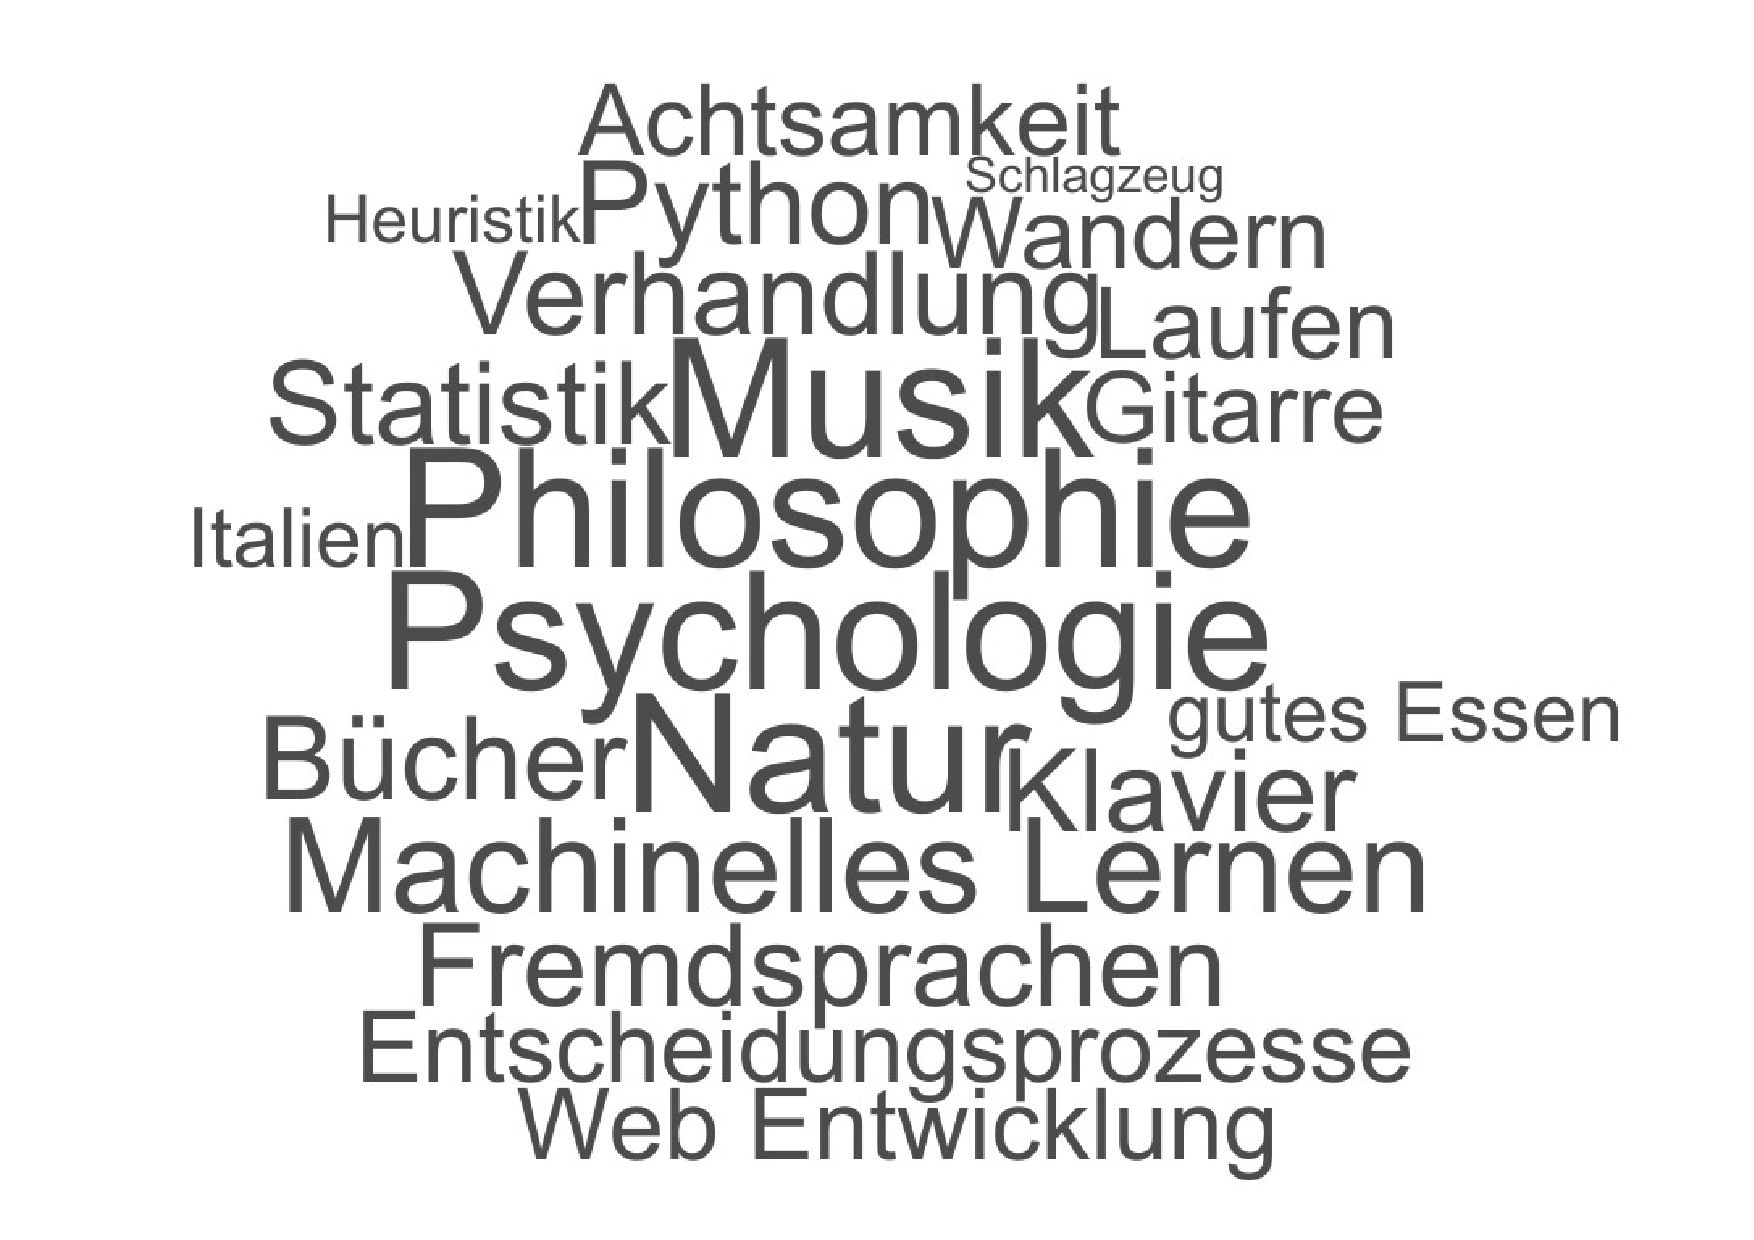
\includegraphics[trim=3cm 1cm 2cm 1cm, clip,scale=0.17]{../../img/wordcloudGER.pdf}
  \end{center}
  \vspace*{\fill}
\end{minipage}
%%%%%%%%%%%%%%%%%%%%%%%%%%%%%%%%%%%%%%%%%%%%%%%%%%%%%%%%%%%%%%%%%%%%%%%%%%%%%%%%%%%%
\hfill
%%%%%%%%%%%%%%%%%%%%%%%%%%%%%%%%%%%%%%%%%%%%%%%%%%%%%%%%%%%%%%%%%%%%%%%%%%%%%%%%%%%%%
\begin{minipage}{0.71\textwidth}
	{\fontsize{30pt}{62pt}\color{gray} \selectfont {Silvio}{\textbf{Schwarz}}}\\
	{\fontsize{14pt}{24pt}\color{pblue} \selectfont Geowissenschaftler \color{lightgray} (B.Sc.)}\\
	\hrule
	\vspace*{-2mm}
	\section*{\fontsize{18pt}{24pt}\selectfont \color{pblue} Ausbildung}
	\textbf{Weiterbildung GIS und Webmapping} \hfill  02.2022  - 10.2022 (8 Monate)\\
	GIS Akademie, Berlin
	\begin{itemize}
		\item ArcGIS
		\item QGIS
		\item PostgreSQL Datenbanken
	\end{itemize}\leavevmode\\
		\textbf{Geowissenschaften (M.Sc.)} \hfill  10.2011  - 09.2019 (8 Jahre)\\
		 Universität Potsdam \hfill~90/120 LP abgeschlossene Studienleistung\\
		Vertiefung:~Geophysik, Machine Learnin\\
		Abschlussarbeit:\\ 1) Forecasting Macroseismic Intensities: A Sensitivity Study of a Bayesian Approach. 2014-2016 \\
		2) Classification of eruptive tremor sources during the 2014-2015 Holuhraun sequence, Iceland. 2019\\
		
		\textbf{\href{https://www.dropbox.com/s/297g1chiby8mrd3/Bachelor-Certificate.pdf?dl=0}{Bachelor of Science: Geowissenschaften}} \hfill 10.2008 - 09.2011 (3 Jahre)\\	Universität Potsdam\\
		{Geologie, Mathematik, Physik, Chemie}\\
		{Abschlussarbeit}: \href{https://www.dropbox.com/s/3kngo4hpb0c47ww/Bachelorarbeit.pdf?dl=0}{{Simulation von Bodenbewegungsszenarien von Starkbeben}} \\
		
		\textbf{\href{https://www.dropbox.com/s/nsgmvy7o64xb9si/Abiturzeugnis.pdf?dl=0}{Abitur}} \hfill 08.2000  - 06.2008 (8 Jahre) \\Klosterschule Roßleben (staatl. Gymnasium)\\
		{Mathematik}, {Geographie}\\
		{Abschlussarbeit}: Naturkatastrophen und ihr Einfluss auf das Leben in der Gegenwart
\\
	\hrule
	%%%%%%%%%%%%%%%%%%%%%%%%%%%%%%%%%%%%%%%%%%%%%%%%%%%%%%%%%%%%%%%%%%%%%%%%%%%%%%%%%
	\section*{\fontsize{18pt}{24pt}\selectfont \color{pblue} Erfahrung}
		\textbf{studentische Hilfskraft}\hfill 05.2019  - 10.2019 (6 Monate)\\Universität Potsdam, Arbeitsgruppe Allgemeine Geophysik
		\begin{itemize}
			\item Charakterisierung von Tremorquellen der Holuhraun Eruption, Island
		\end{itemize}
	%	{Betreuung}: Prof. Dr. Eva Eibl
	
	\vspace{\spacingWork}
	
%			\begin{minipage}[t]{\minipageSmall\textwidth}
%				\raggedleft
%				11/2017 - 03/2018\\(5 Monate)
%			\end{minipage}
%			\hfill
%			\begin{minipage}[t]{\minipageBig\textwidth}
%				\textbf{Werksstudent}\hfill \href{https://assecor.de/}{\color{pblue}DB Dialog}\\
%				support passenger rights
%			\end{minipage}

	%		\vspace{\spacingWork}
	%		
	%				\begin{minipage}[t]{0.25\textwidth}
	%				\centering
	%				01/2013\\ -\\ 04/2013 \\(3 Monate)
	%				\end{minipage}
	%				\hfill
	%				\begin{minipage}[t]{\minipageBig\textwidth}
	%				\textbf{Praktikum}\footnote{cancelled due to illness}\hfill	
	%				\href{https:///www.munichre.com/}{\color{pblue}Munich Re}\\
	%				Improvement of GMPE\\
	%				\textbf{Betreuung}}: \href{mailto:MKaeser@munichre.com}{\color{pblue}Prof. Dr. Martin Käser}%https://www.geophysik.uni-muenchen.de/Members/kaeser/cv
	%				\end{minipage}

%	\vspace{\spacingWork}
		\textbf{Werksstudent}\hfill 08.2014 - 06.2015 (11 Monate)\\ Assecor GmbH, Berlin
		\begin{itemize}
			\item Dokumentation des Berliner Stromnetzes in einem Netzinformationssystem für Vattenfall Europe Sales GmbH
		\end{itemize}
		
	\vspace{\spacingWork}
	
		\textbf{Werksstudent}\hfill 11.2013 - 03.2014 (5 Monate)\\ Assecor GmbH, Berlin
		\begin{itemize}
			\item Migration der IT Infrastruktur für BIOTRONIK SE \& Co. KG
		\end{itemize}
		
	\vspace{\spacingWork}
	
		\textbf{Master Praktikum}\hfill 09.2012 - 11.2012 (3 Monate)\\ Wolfram$\mid$Alpha, Illinois, USA
		\begin{itemize}
			\item Entwicklung von geophysikalischen Inhalt für Wolfram$~\mid~$Alpha\hfill \href{https://www.wolframalpha.com/input/?i=moment+magnitude}{\color{pblue}Beispiel}
		\end{itemize}
		%	{Betreuung}: Dr. Björn Zimmermann \& Dr. Michael Trott
		
	\vspace{\spacingWork}
	
		\textbf{studentische Hilfskraft}\hfill 06.2011 - 08.2012 (1 Jahr 3 Monate)\\Universität Potsdam
		\begin{itemize}
			\item SSHAC LEVEL 3 PSHA Modellerstellung und Beratung
			\item 1-wöchige Beratung für Prof. Julian J. Bommer, Imperial College London
		\end{itemize}

	%	{Betreuung}: Prof. Frank Scherbaum

	\vspace{\spacingWork}

		\textbf{Bachelor Praktikum}\hfill 03.2011 (1 Monat)\\ Universität Leipzig
		\begin{itemize}
			\item Wartung des seismologischen Netzwerkes von Sachsen
		\end{itemize}
		%{Betreuung}: Dipl. Geophys. S. Funke
\end{minipage}
%\vspace*{\fill}
\end{document}